
\documentclass[runningheads]{llncs}

%\documentclass[11pt,a4paper]{article} %UKenglish,
%\textheight24cm
%\textwidth16cm
%\topmargin-5mm
%\oddsidemargin0cm
%\evensidemargin0cm

\usepackage{enumerate}
\usepackage{textcomp}
\usepackage{url}
\usepackage{graphicx}
\usepackage{amssymb}
\usepackage{amsmath}
%\usepackage{amsthm}
\usepackage{verbatim}
%\usepackage{subcaption}
\usepackage[utf8]{inputenc}
\usepackage{color}

\newcommand{\ifdraft}[1]{#1}
\definecolor{aocolour}{rgb}{0.7,0.8,1}
\newcommand{\ao}[1]{\ifdraft{\noindent\colorbox{aocolour}{A.O.: #1}}}

\newcommand{\xra}[1]{\overset{#1}{\rightsquigarrow}}

\newcommand{\set}[2]{\{ \, #1 \mid #2 \, \}}
\newcommand{\setbig}[2]{\big\{ \: #1 \;\big|\; #2 \: \big\}}
\renewcommand{\emptyset}{\varnothing}
\renewcommand{\epsilon}{\varepsilon}

\DeclareMathOperator{\osc}{\textup{osc}}

%\newtheorem{lemma}{Lemma}
%\newtheorem{theorem}{Theorem}
%\newtheorem{definition}{Definition}
%\newtheorem{example}{Example}
%\newtheorem{corollary}{Corollary}


\begin{document}


\sloppy

%\begin{comment} % *********** for LNCS ************
\title{Rational index of languages with bounded dimension of parse trees\footnote{%
This research was supported by the Russian Science Foundation, project 18-11-00100.}}

\author{Ekaterina Shemetova\footnote{%
Department of Mathematics and Computer Science, St. Petersburg State University, 
7/9 Universitetskaya nab., Saint Petersburg 199034, Russia.}
\footnote{%
St. Petersburg Academic University, 
ul. Khlopina, 8, Saint Petersburg 194021, Russia.}
\footnote{%
JetBrains Research,
Primorskiy prospekt 68-70, Building 1, St. Petersburg, 197374, Russia.}
\and
Alexander Okhotin\footnotemark[2]
\and
Semyon Grigorev\footnotemark[2] \footnotemark[4]
}
%\end{comment}

\title{Rational index of languages with bounded dimension of parse trees\thanks{%
	Research supported by the Russian Science Foundation, project 18-11-00100.}
}

\author{Ekaterina Shemetova\inst{1,2,3}
\and
Alexander Okhotin\inst{1}
\and
Semyon Grigorev\inst{1,3}
}

\institute{%
	Department of Mathematics and Computer Science, St. Petersburg State University, 
	7/9 Universitetskaya nab., Saint Petersburg 199034, Russia
\and
	St. Petersburg Academic University, 
	ul. Khlopina, 8, Saint Petersburg 194021, Russia
\and
	JetBrains Research,
	Primorskiy prospekt 68-70, Building 1, St. Petersburg, 197374, Russia
}


\maketitle


\begin{abstract}
The rational index $\rho_L$ of a language $L$ is an integer function,
where $\rho_L(n)$ is the maximum length of the shortest string in $L \cap R$,
over all regular languages $R$ recognized by $n$-state nondeterministic finite automata (NFA).
This paper investigates the rational index of languages
defined by (context-free) grammars with bounded tree dimension,
and shows that it is of polynomial in $n$.
More precisely, it is proved that for a grammar with tree dimension bounded by $d$,
its rational index is $O(n^{2d})$,
and that this estimation is precise,
as there exists a grammar with rational index $\Theta(n^{2d})$.

\textbf{Keywords.}
Dimension of a parse tree; rational index; CFL-reachability; parallel complexity; context-free languages; Datalog programs.
\end{abstract}





\section{Introduction}\label{section_introduction}

The notion of a rational index was introduced by Boasson, Courcelle and Nivat~\cite{RatBasic}
as a complexity measure for context-free languages.
The rational index $\rho_L$ of a language $L$ is an integer function,
where $\rho_L(n)$ is the maximum length of the shortest string in a language of the form $L \cap R$,
where $R$ is a regular language recognized by $n$-state nondeterministic finite automata (NFA),
and the maximum is taken over all such languages $R$.
The rational index plays an important role
in determining the parallel complexity of such practical problems
as the CFL-reachability problem
and the more general Datalog query evaluation.

The rational index of a context-free language $L$ is an integer function $\rho_L$,
where $\rho_L(n)$ is the maximum length of the shortest string in the intersection of $L$
with a regular language $R$ recognized by a finite automaton with $n$ states,

The \emph{CFL-reachability problem} is stated as follows:
given a context-free grammar $G$
and an NFA $A$ over the same alphabet,
determine whether $L(G) \cap L(A)$ is non-empty.
With $A$ is regarded as a labelled graph,
%a directed edge-labeled graph $D$ and a pair of nodes $u$ and $v$,
%determine whether there is a path from $u$ to $v$ labeled with a string in $L(G)$.
%That is, CFL-reachability 
this is a kind of graph reachability problem
with path constraints given by context-free languages.
This is an important problem used in static code analysis~\cite{RepsBasic}
and graph database query evaluation~\cite{Yannakakis}.

%Unlike context-free language recognition,
%which is in NC for a fixed context-free grammar,
The CFL-reachability problem is P-complete
already for a fixed context-free grammar~\cite{PCompl}.
%Practically, it means that there is no efficient parallel algorithm
%for solving this problem (unless P $\neq$ NC). 
The question on the parallel complexity of this problem
was investigated by Ullman and Van Gelder \cite{Ullman}
in a much more general case,
with a rich logic for database queries instead of grammars,
and it was proved that under
an assumption called the \emph{polynomial fringe property}
the problem is decidable in NC~\cite{Ullman}.
In the special case of grammars,
the result of Ullman and Van Gelder \cite{Ullman}
gives an NC$^2$ algorithm for the CFL-reachability problem,
under the assumption that the grammar's rational index is polynomial.
% implicit in Corollary 7.1.

%was extensively investigated by the deductive database community~\cite{ChainQ,Ullman}.
%that if the context-free language has a polynomial rational index
%The polynomial fringe property is equivalent to having the polynomial rational index:
%for a context-free language $L(G)$ having the polynomial rational index $\rho_L(n) = poly(n)$,
%where $poly(n)$ is some polynomial, is the same as for corresponding chain query
%to have the polynomial fringe property.

%This motivates further study of
Theoretical properties of the rational index
have received some attention in the literature.
Pierre and Farinone~\cite{GreibRat} proved that for every algebraic number $\gamma$,
a language with the rational index in $\Theta(n^\gamma)$ exists.
An upper bound on the rational index,
shown by Pierre~\cite{CFRat}, is $2^{\Theta(n^2/\ln n)}$,
and this bound is reached on the Dyck language on two pairs of parentheses.
For several important subfamilies of grammars,
such as the linear and the one-counter languages,
there are polynomial upper bounds on the rational index,
which imply that the CFL-reachability problem is in NC$^2$;
they can be proved to lie in NL
by direct methods not involving the rational index~\cite{labelledGraphs,LReach}.

In this paper we investigate the rational index of a generalization of linear languages:
the \emph{languages of bounded tree dimension},
that is, those defined by grammars
with a certain limit on branching in the parse trees;
see Luttenberger and Schlund~\cite{LuttenbergerSchlund} for a survey of tree dimension.
Linear languages are languages of tree dimension 1,
the their rational index is known to be $O(n^2)$~\cite{RatBasic}.
The result of this paper is that languages of tree dimension bounded by $d$
have rational index $O(n^{2d})$,
and furthermore, for every $d$, there is a language of tree dimension bounded by $d$
with rational index $\Theta(n^{2d})$.
%$that has the rational index at least $n^{2d}/2^c$.






\section{Definitions}\label{section_definitions}

A \textit{(context-free) grammar} is a quadruple $G = (\Sigma, N, R, S)$,
where $\Sigma$ is an alphabet;
$N$ is a set of nonterminal symbols;
$R$ is a set of rules, each of the form $A \to \alpha$,
with $A \in N$ and $\alpha \in (\Sigma \cup N)^*$;
and $S \in N$ is the start symbol.
A parse tree is a tree, in which 
every leaf is labelled with a symbol from $\Sigma$,
while every internal node is labelled with a nonterminal symbol $A \in N$
and has an associated rule $A \to X_1 \ldots X_\ell \in R$,
so that the node has $\ell$ ordered children labelled with $X_1, \ldots, X_\ell$.
The language defined by each nonterminal symbol $A \in N$, denoted by $L_G(A)$,
is the set of all strings $w \in \Sigma^*$,
for which there exists a parse tree,
with $A$ as a root
and with the leaves forming the string $w$,
The language defined by the grammar is $L(G)=L_G(S)$.

A grammar $G$ is said to be is in the \textit{Chomsky normal form},
if all rules of $R$ are of the form
$A \to BC$, with $B, C \in N$, or of the form $A \to a$, with $a \in \Sigma$. 

\begin{comment}
The set of all context-free languages is identical to the set of languages accepted by pushdown automata (PDA). \textit{Pushdown automaton} is a 7-tuple $M = (Q, \Sigma, \Gamma, \delta, q_0, Z, F)$, where $Q$ is a finite set of states, $\Sigma$ is a input alphabet, $\Gamma$ is a finite set which is called the stack alphabet, $\delta$ is a finite subset of $Q \times (\Sigma \cap \{\varepsilon\}) \times \Gamma \times Q \times \Gamma^*$,
$q_{0}\in Q$ is the start state, $Z \in \Gamma$ is the initial stack symbol and
$F\subseteq Q$ is the set of accepting states.
\end{comment}

A \textit{nondeterministic finite automaton} (NFA) is a quintuple
$\mathcal{A}=(\Sigma, Q, Q_0, \delta, F)$, where $Q$ is a finite set of states,
$\Sigma$ is a finite set of input symbols,
$Q_0 \subseteq Q$ is the set of initial states,
$\delta \colon Q \times \Sigma \to 2^Q$ is the transition function,
$F \subseteq Q$ is the set of accepting states.
%\textit{Deterministic finite automaton} is a NFA with the following restrictions: each of its transitions is uniquely determined by its source state and input symbol, and reading an input symbol is required for each state transition.
It accepts a string $w=a_1 \ldots a_n$ if there is a sequence of states $q_0, \ldots, q_n \in Q$
with $q_0 \in Q_0$, $q_i \in \delta(q_{i-1}, a_i)$ for all $i$, and $q_n \in F$.
The language of all strings accepted by $\mathcal{A}$ is denoted by $L(\mathcal{A})$.

For a language $L$ over an alphabet $\Sigma$,
its rational index $\rho_L$ is a function defined as follows:
\begin{equation*}
	\rho_L(n)
		=
	\max_{\substack{\mathcal{A} \text{:NFA with }n\text{ states} \\ L \cap L(\mathcal{A}) \neq \emptyset}}
	\;
	\min_{w \in L \cap L(\mathcal{A})}|w|
\end{equation*}


\paragraph{Tree dimension.} 
For each node $v$ in a parse tree $t$,
its \emph{dimension} $\dim v$ is an integer
representing the amount of branching in its subtree.
It is defined inductively: %on the structure of subtrees.
a leaf $v$ has dimension $0$.
%\begin{itemize}
%\item if $v$ is a leaf, then $dim(v)$ = 0
For an internal node $v$, if one of its children $v_1, v_2, \ldots, v_k$, with $k \geqslant 1$,
has a greater dimension than all the others,
then $v$ has the same dimension,
and if there are multiple children of maximum dimension,
then the dimension of $v$ is greater by one.
\begin{equation*}
	\dim v
		=
	\begin{cases}
	\max_{i \in \{1, \ldots, k\}} \dim v_i
		&\text{if there is a unique maximum} \\
	\max_{i \in \{1, \ldots, k\}} \dim v_i +1
		&\text{otherwise}
	\end{cases}
\end{equation*}
The dimension of a parse tree $t$, denoted by $\dim t$, is the dimension of its root. 
%It is observable from the definition that the dimension of a tree $t$
%This is the height of the largest perfect binary tree,
%obtained from $t$ by contracting edges and identifying vertices.

%A tree of dimension $dim(t) = 2$ is illustrated in Figure~\ref{oscbtree}.

\begin{definition}[Grammars of bounded tree dimension]
A grammar $G$ is of $d$-bounded tree dimension
if every parse tree $t$ of $G$ has $\dim t \leqslant d$,
where $d$ is some constant.
This constant is called the dimension of $G$, denoted by $\dim G=d$.
\end{definition}

Classical transformation to the Chomsky normal form
preserves the class of grammars of $d$-bounded tree dimensions.
Languages defined by such grammars are called \emph{languages of $d$-bounded tree dimension}.


\begin{comment}
\paragraph{Context-free language reachability.} 
A \textit{directed labeled graph} is a triple $D = (Q, \Sigma, \delta)$, where $Q$ is a finite set of nodes, $\Sigma$ is a finite set of alphabet symbols,
and $\delta \subseteq Q \times \Sigma \times Q$ is a finite set of labeled edges. Let $L(D)$ denote a graph language a regular language, which is recognized by the NFA $(Q,\Sigma ,\delta ,Q, Q)$ obtained from $D$ by setting every state as inial and accepting.


Let $i\pi j$ denote a unique path between nodes $i$ and $j$ of the input graph and $l(\pi)$ denote a unique string obtained by concatenating edge labels along the path $\pi$. Then the CFL-reachability can be defined as follows.
\begin{definition}[Context-free language reachability]
Let $L \subseteq \Sigma^*$ be a context-free language and $D = (Q, \Sigma, \delta)$ be a directed labeled graph. Given two nodes $i$ and $j$ we say that $j$ is \textit{reachable} from $i$ if there exists a path $i \pi j$, such that $l(\pi) \in L$. 
\end{definition}
There are four varieties of CFL-reachability problems: all-pairs problem, single-source problem, single-target problem and single-source/single-target problem \cite{RepsBasic}. In this paper we consider single-source/single-target problem. 
\end{comment}





\section{Upper bound on the rational index} % of languages of bounded tree dimension}

\begin{comment}
Before we estimate the value of the rational index for languages of bounded tree dimension,
we need to prove the following.

\begin{lemma}\label{lem:treeheight}
Let $G = (\Sigma, N, R, S)$ be a grammar in the Chomsky normal form,
and let $\mathcal{A}=(\Sigma, Q, Q_0, \delta, F)$ be an NFA with $n$ states.
Let $w$ be the shortest string in $L(G)\cap L(\mathcal{A})$.
Then the height of every parse tree for $w$ in $G$ does not exceed $|N|n^2$.
\end{lemma}
\begin{proof}
Consider the grammar for $L(G)\cap L(\mathcal{A})$
constructed from $G$
using the classical construction by Bar-Hillel et al.~\cite{BarHillel}.
It is defined as $G' = (\Sigma, N' \cup \{S'\}, R', S')$,
where $N'=N \times Q \times Q$,
and $R$ contains the following rules.
\begin{align*}
	(A, p, q) &\to (B, p, r) (C, r, q),
		 && \text{for all } A \to BC \in R \text{ and } p, r, q \in Q
		 	\\
	(A, p, q) &\to a,
		 && \text{for all } A \to a \in R \text{ and } p, q \in Q \text{ with } q \in \delta(p, a)
		 	\\
	S' &\to (S, p, q),
		 && \text{for all } p \in Q_0 \text{ and } q \in F
\end{align*}
%A triple $(A, i, j)$ is \textit{realizable} if and only if there is a path $i\pi j$
%such that $A \stackrel {*}{\to } l(\pi)$ for some nontermimal $A \in N$.
Then the parse tree $t_G$ for $w$ in $G$ can be converted into a parse tree $t_{G'}$ for $w$ in $G'$,
which has the same structure and the same first components of all labels,
whereas the attached pairs of states
correspond to a segment of the accepting computation of $\mathcal{A}$ on $w$.
%Notice that every node of $t_{G'}$ is realizable triple.
In particular, the height of $t_G$ is equal to the height of $t_{G'}$.

Assume that the height of $t_{G'}$ exceeds $|N|n^2$,
and consider an offending path from the root of the parse tree to a leaf,
of length greater than $|N|n^2$.
As there are $|N'|=|N|n^2$ unique node labels,
this path has at least two nodes with the same label.
Then the segment of the path between these two nodes can be contracted,
resulting in a valid parse tree for a string shorter than $w$.
%This means that the parse tree for $w$
%contains at least one subtree $t$ with label $(A, i, j)$ at the root,
%which has a subtree $t'$ with the same label.
%Then we can change $t$ with $t'$ and get a new string $w'$,
%which is shorter than $w$.
This contradicts $w$'s being the shortest.
\qed
\end{proof}

From Lemma~\ref{lem:treeheight} one can deduce an alternative proof
of the fact that the rational index of linear languages is in $O(n^2)$~\cite{RatBasic}:
the number of leaves in a parse tree in linear grammar is proportional to its height,
and thus it is in $O(n^2)$.
\end{comment}

\begin{lemma}\label{dimlemma}
Let $G = (\Sigma, N, R, S)$ be a grammar in the Chomsky normal form,
and let $\mathcal{A}$ be an NFA with $n$ states.
Let $A \in N$ and $p, q \in Q$.
Let $w$ be the shortest string in $L_G(A)$,
such that $\mathcal{A}$ can read $w$ starting from state $p$
and ending in state $q$.
%$w \in L_G(A)$ and $q \in \delta(p, w)$,
Let $t$ be a parse tree of $w$ as $A$,
and let $d$ be the dimension of $t$.
Then, $|w| \leqslant |N|^d n^{2d}$.
\end{lemma}
\begin{proof}
The proof is by induction on the dimension of $t$.

\textbf{Basis:} $\dim t=0$.
Then, $t$ should use a rule $A \to a$, and $w=a$.
The desired inequality holds as an equality $|w| = 1 = |N|^0 n^0$.

\textbf{Inductive step:} dimension $d-1 \to d$.
Let $t$ have dimension $d$,
and consider the path from the root of $t$ passing through nodes of dimension $d$.
If both children of the root of $t$ have dimension $d-1$,
then this path consists of a single node;
otherwise, one of the children of of the root of $t$ has dimension $d$,
and the other has dimension less than $d$,
and the path continues to the child of dimension $d$, etc.
Let the path contain $h$ edges,
and let $A_0, A_1, \ldots, A_h$ be the nonterminals in the labels of nodes on this path,
with $A_0=A$.
%Then the one with dimension $d$ may also have one child of dimension $d$, etc.

At each node of this path except the last one,
a subtree of dimension less than $d$
spawns off to the left or to the right,
whereas the last node on this path has two children of dimension $d-1$.
Let $s_1, \ldots, s_k$ be the subtrees spawned off to the left,
let $B_i \in N$ be the root of each $s_i$,
and let $u_i$ be the substring corresponding to $s_i$.
Similarly, let $t_1, \ldots, t_\ell$ be the subtrees spawned off to the right,
with each $t_i$ having a root $C_i$ and corresponding to a substring $v_i$.
Then $k+\ell=h$.
Let the last node on the path have two children labelled with $B_{k+1}$ and $C_{\ell+1}$,
with the corresponding substrings $u_{k+1}$ and $v_{\ell+1}$.
Then, $w = u_1 \ldots u_k u_{k+1} v_{\ell+1} v_\ell \ldots v_1$,
as illustrated in Figure~\ref{dimupper}.

Consider the computation of $\mathcal{A}$ on $w$,
which starts in $p$ and ends in $q$,
and consider the following intermediate states in this computation:
let $p_i$ be the state after reading each $u_i$,
and let $q_i$ be the state before reach each $v_i$.
Also let $p_0=p$ and $q_0=q$ for uniformity.
Then each string $u_i$ is a string in $L_G(B_i)$,
which $\mathcal{A}$ can read starting in $p_{i-1}$ and finishing in $p_i$;
this must be the shortest string with this property,
for otherwise $w$ could be shortened by replacing $u_i$ with a shorter one.
By the same reasoning, each $v_i$ is the shortest string in $L_G(C_i)$,
on which $\mathcal{A}$ has a computation that begins in $q_i$ and ends in $q_{i-1}$.
Then, by the induction hypothesis,
$|u_i|,|v_i| \leqslant |N|^{d-1}n^{2(d-1)}$ for all applicable $i$.
This upper bound holds for $k+\ell+2=h+2$ subtrees
shown in Figure~\ref{dimupper}.
 
Next, it is claimed that the number $h+2$
is bounded by $|N| \cdot n^2$.
Suppose, for the sake of a contradiction,
that $h+2 > |N| \cdot n^2$.
Consider the nodes $A_0, A_1, \ldots, A_h$ on the main path,
followed by the left child $B_{k+1}$.
Each of them has a corresponding substring of the form $u_{i+1} \ldots u_{k+1} v_{k+1} \ldots v_{j+1}$
(or $u_{k+1}$ in the case of $B_{k+1}$),
and the computation of $\mathcal{A}$ on $w$
begins reading this substring in the state $p_i$ and ends reading it in the state $q_j$.
Accordingly, each of these $h+2$ nodes
has an associated triple that consists of a nonterminal symbol and two states.
In total, there are $|N| \cdot n^2$ distinct triples of this form.
Since $h+2 > |N| \cdot n^2$ by the assumption,
some triple must occur on this path multiple times.
Then the segment of the path between these two nodes can be contracted,
resulting in a valid parse tree of a string shorter than $w$ as $A$,
while the computation of $\mathcal{A}$ on $w$
is accordingly contracted to remove two fragments,
resulting in a computation of $\mathcal{A}$ on a shorter string.
This contradicts the assumption
that $w$ is the shortest string with this property,
and thus confirms that $h+2 \leqslant |N| \cdot n^2$.

Then the length of $w$ is bounded as follows.
\begin{equation*}
	|w|
		=
	\sum_i |u_i| + \sum_i |v_i|
		\leqslant
	(h+2) \cdot |N|^{d-1} n^{2(d-1)}
		\leqslant
	|N| \cdot n^2 \cdot |N|^{d-1} n^{2(d-1)}
		=
	|N|^d n^{2d}
\end{equation*}
\qed
\end{proof}

\begin{figure}[t]
	\centering
	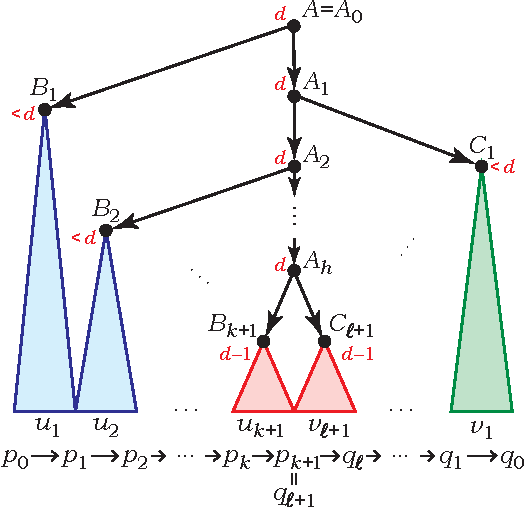
\includegraphics[scale=0.9]{pictures/rational_index_upper_bound}
	\caption{A parse tree, with a path from the root passing through nodes of dimension $d$.}
	\label{dimupper}
\end{figure}

\begin{theorem}
\label{oscbnddim}
Let $G$ be a grammar of $d$-bounded tree dimension,
and let $\mathcal{A}$ be an NFA with $n$ states.
Then the length of the shortest string in $L(G) \cap L(\mathcal{A})$ is at most $|G|^d n^{2d}$,
where $|G|$ is sum of lengths of all rules of the grammar.
\end{theorem}
\begin{proof}
A given grammar $G$ is first transformed to the Chomsky normal form,
resulting in a grammar with the same bound on the tree dimension
and with at most $|G|$ nonterminal symbols.

Let $w$ be the shortest string in $L(G) \cap L(\mathcal{A})$,
and let $q_0 \in Q_0$ and $r \in F$ be the first and the last states
in the computation of $\mathcal{A}$ on $w$.
Then, $w$ is the shortest string in $L_G(S)$,
which $\mathcal{A}$ can read starting in the state $q_0$
and ending in the state $r$.
Then, by Lemma~\ref{dimlemma},
the length of $w$ is at most $|G|^d n^{2d}$.
\qed
\end{proof}






\section{Lower bound on the rational index}\label{section_lower_bound} % of languages of bounded tree dimension}

The upper bound $O(n^{2d})$ on the rational index of a language
defined by grammar with tree dimension bounded by $d$
has a matching lower bound $\Omega(n^{2d})$.
It is first established for a convenient infinite set of values of $n$,
to be extended to arbitrary $n$ in the following.

\begin{lemma}\label{lowerlemma}
For every $d \geqslant 1$,
there is a grammar $G$ of bounded tree dimension $d$,
such that for every $n \geqslant 2^{d+1}$ divisible by $2^d$
there is an $n$-state NFA $\mathcal{A}$,
such that the shortest string $w$ in $L(G) \cap L(\mathcal{A})$
is of length at least $\frac{1}{2^{d^2 + 3d - 3}} n^{2d}$.
\end{lemma}
\begin{proof}
The grammar and the automaton are constructed inductively on $d$,
for every $d$ and only for $n$ divisible by $2^d$.
Each constructed NFA shall have a unique initial state,
which is also the unique accepting state.

\textbf{Basis.} $dim(G) = 1$.
The family of languages having dimension $d = 1$
coincides with the family of linear languages.
Let $G$ be a linear grammar with the rules $S \to aSb \ | \ ab$,
which defines the language $L(G) = \set{a^i b^i}{i \geqslant 1}$. 

For every $n \geqslant 4$ divisible by $2^d=2$,
let $\ell = \frac{n}{2}$, $m=\frac{n}{2} + 1$.
Then $\ell$ and $m$ are coprime integers.
Define an NFA $\mathcal{A}$ over the alphabet $\{a, b\}$,
which consists of two cycles
sharing one node, $q_0$,
which is both the initial and the unique accepting state.
The cycle of length $\ell$ has all transitions by $a$, and the other by $b$,
as shown in Figure~\ref{worstd_1}.
The automaton has $\ell+m-1=n$ states.

Every string in $L(G) \cap L(\mathcal{A})$
is of the form $a^i b^i$, with $i \geqslant 1$.
For the automaton to accept it,
$i$ must be divisible both by $\ell$ and by $m$.
Since the cycle lengths are relatively prime,
the shortest string $w$ with this property has $i=\ell m$,
and is accordingly of length $2\ell m$.
Its growth with $n$ is estimated as follows.
\begin{equation*}
	|w|
		=
	2\ell m
		=
	2 \frac{n}{2} \cdot (\frac{n}{2} + 1)
		=
	\frac{1}{2} n^2 + n
\end{equation*}
This example is well-known to the community~\cite{HellingsCFPQ,Yannakakis}. 

\begin{figure}[t]
\centering
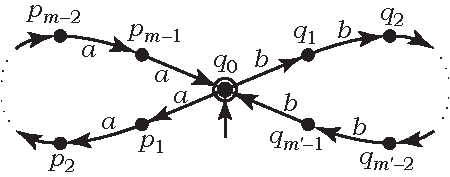
\includegraphics[scale=0.9]{pictures/rational_index_A1.pdf}
\caption{Worst-case NFA $\mathcal{A}$ for grammar $G$ of bounded dimension $d=1$}
\label{worstd_1}
\end{figure}

\textbf{Inductive step.} $dim(G) = d$.

By the induction hypothesis,
there is a grammar $\widehat{G} = (\widehat{\Sigma}, \widehat{N}, \widehat{R}, \widehat{S})$
of bounded dimension $dim(\widehat{G}) = d-1$,
which satisfies the statement of the lemma.
The new grammar $G = (\Sigma, N, R, S)$ of dimension $d$
is defined over the alphabet 
$\Sigma = \widehat{\Sigma} \cup \{a, b, c\}$,
where $a, b, c \not\in \widehat{\Sigma}$ are new symbols.
It uses nonterminal symbols
$N = \widehat{N} \cup \{S, A\}$,
adding two new nonterminals $A, S \not\in \widehat{N}$ to those in $\widehat{G}$,
where $S$ is the new initial symbol.
Its set of rules includes all rules from $\widehat{G}$
and the following new rules.
\begin{align*}
	S &\to A S c \ | \ A c \\
	A &\to a A b \ | \ a \widehat{S} b
\end{align*}

\begin{figure}[t]
\centering
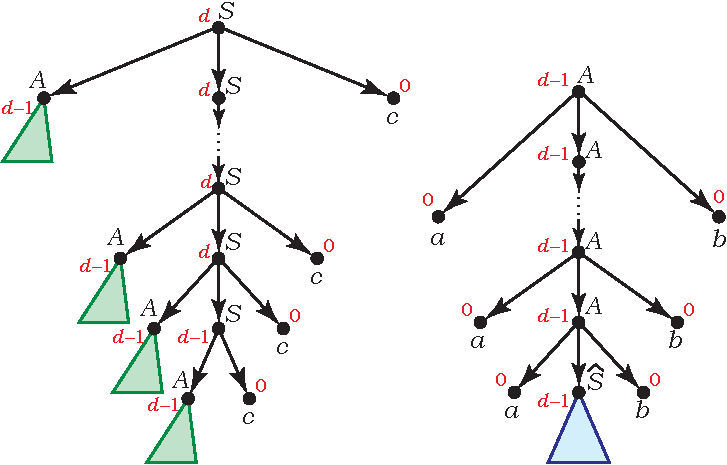
\includegraphics[scale=0.9]{pictures/rational_index_parse_tree_S_A.pdf}
\caption{Parse trees for $S$ and for $A$, annotated with dimensions of their vertices}
\label{dimsubtree}
\end{figure}

To see that the dimension of the new grammar is greater by 1 than the dimension of $\widehat{G}$,
%$dim(G) = dim(\widehat{G}) + 1 = d$.
first consider the dimension of any parse tree $t$ with the root labeled by the nonterminal $A$,
shown in Figure~\ref{dimsubtree}(right).
The dimension of the $\widehat{S}$-subtree at the bottom
is at most $d-1$ by the properties of $\widehat{G}$.
This dimension is inherited by all $A$-nodes in the tree,
because their remaining children are leaves.
%Multiple applications of the rule $A \to a A b$
%do not increase the dimension of the parse tree,
%because the dimensions of nodes labeled with $a$, $b$ are equal to $0$.

Now consider the dimension of a complete parse tree $t$ with the start symbol $S$ in the root,
as in Figure~\ref{dimsubtree}(left).
All $A$-subtrees in this tree have dimension at most $d-1$.
Then the bottom $S$-subtree, which uses the rule $S \to Ac$,
also has dimension at most $d-1$.
Every $S$-subtree higher up in the tree uses a rule $S \to ASc$,
and its dimension is at most $d$,
because getting a higher dimension would require two subtrees of dimension $d$,
which is never the case.
%As there is no unique maximum, $dim(t) = \max_{i} (v_i) + 1 = d - 1 + 1 = d$.
%Notice that only one application of the rule $S \to A S c$ increases the dimension of $t$,
%whereas further applications do not make any effect on the dimension of parse tree.

Now, for every $n \geqslant 2^{d+1}$ divisible by $2^d$,
the goal is to construct an $n$-state NFA over the alphabet $\Sigma$,
so that the shortest string $w$ in $L(G) \cap L(\mathcal{A})$.
Since the number $\frac{n}{2}$ is at least $2^d$ and is divisible by $2^{d-1}$,
the induction hypothesis for the grammar $\widehat{G}$
asserts that there is an NFA
$\widehat{\mathcal{A}} = (\widehat{Q}, \widehat{\Sigma}, \widehat{\delta}, \widehat{q}_0, \{\widehat{q}_0\})$,
with $\frac{n}{2}$ states,
with the shortest string $\widehat{w}$ in $L(\widehat{G}) \cap L(\widehat{\mathcal{A}})$
of length $\frac{1}{2^{(d-1)^2 + 3(d-1) - 3}} (\frac{n}{2})^{2(d-1)}$.

The desired $n$-state NFA $\mathcal{A} = (\Sigma, Q, q_0, \delta, \{q_0\})$
is constructed as follows.
Let $\ell = \frac{n}{4}$ and $m=\frac{n}{4} + 1$, these are two coprime integers.
The set of states of $\mathcal{A}$
contains all $\frac{n}{2}$ states from $\widehat{Q}$,
in which $\mathcal{A}$ it operates as $\widehat{\mathcal{A}}$,
and $m+\ell-1=\frac{n}{2}$ new states forming
a cycle of length $\ell$ and a chain of length $m$,
which share a state.
\begin{equation*}
	Q = \widehat{Q} \cup \{p_1, \ldots, p_{\ell-1}, q_0, \ldots, q_{m-1}\}
\end{equation*}
The new initial state $q_0$ has a transition by $a$
leading to the initial state of $\widehat{\mathcal{A}}$,
from where one can return to $q_1$ by $b$.
\begin{align*}
	\delta(q_0, a) &= \{\widehat{q}_0\}
		\\
	\delta(\widehat{q}_0, b) &= \{q_1\}
\intertext{%
There is a chain of transitions by $a$ from $q_{m-1}$ to $q_0$,
and another chain $b$ in the opposite direction, from $q_1$ to $q_{m-1}$ and back to $q_0$.
}
	\delta(q_i, a) &= \{q_{i-1}\},
		&& \text{with } 1 \leqslant i \leqslant m-1
		\\
	\delta(q_i, b) &= \{q_{i+1}\},
		&& \text{with } 1 \leqslant i \leqslant m-2
		\\
	\delta(q_{m-1}, b) &= \{q_0\}
\intertext{%
There is a cycle by $c$ in the states $q_0, p_1, \ldots, p_{\ell-1}$;
for uniformity, denote $p_0=q_0$.
}
	\delta(p_i, c) &= \{p_{i+1 \bmod \ell}\},
		&& \text{with } 0 \leqslant i \leqslant \ell-1
\end{align*}
The general form of $\mathcal{A}$ is shown in Figure~\ref{dimautomata:generalized}.

\begin{figure}[t]
	\centering
	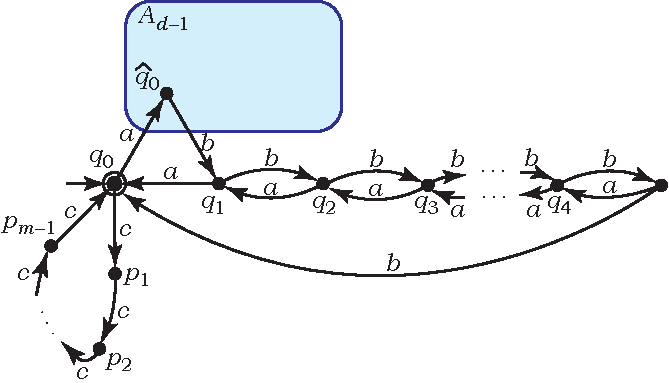
\includegraphics[scale=0.9]{pictures/rational_index_Ad}
	\caption{NFA $\mathcal{A}$ for grammar $G$ of bounded dimension $d$}
	\label{dimautomata:generalized}
\end{figure}

Let $w$ be the shortest string in $L(G) \cap L(\mathcal{A})$.
Consider how $w$ is formed.
Start state is $q_{0}$.
According to the grammar rule $S \to A S c\ \vert \ A c$,
the string $w$ should start with a substring $u$ in $L_G(A)$.
There is the only one outgoing edge labeled with $a$,
so the next state is $\widehat{q}_{0}$.
The next part of $w$ should be a symbol $a$
or a string $v$ in $L(\widehat{G})$.
As there is no outgoing edge labeled with $a$,
the string $v$ is the shortest string in $L(\widehat{G}) \cap L(\widehat{\mathcal{A}})$,
and, hence, $v = \widehat{w}$.
Now the first part of $w$ is $a \widehat{w}$.
To complete a substring derived by the nonterminal $A$,
there is only one possible transition,
which is an edge from $\widehat{q}_{0}$ to $q_1$ labeled with $b$.
The next substring should be symbol $c$ (the rule $S \to A c$) or a string derived by $A$.
The only suitable transition here is from $q_1$ to $q_0$ by $a$,
so a substring in $L(A)$ is started.
Again, to complete the string generated by $A$,
one goes to the state $q_2$,
and $w$ now starts with $a \widehat{w} b a a \widehat{w} b b$.
By the construction of NFA $\mathcal{A}$,
this process continues until one comes to the state $q_0$
without starting a substring derived by the nonterminal $A$
(notice that such substrings are the shortest possible).
Clearly, it happens after $m$ iterations.
Then it is left to read $m$ symbols $c$ by going from $q_0$ to $q_0$.
But $m$ and $\ell$ are coprime, so to balance the number of substrings
derived by the nonterminal $A$
and the number of symbols $c$,
one needs to repeat the first cycle $\ell$ times and the second cycle $m$ times.

Accordingly, the shortest string $w$ has the following structure.
Let $w_i$ be the shortest string
such that there exists computation $q_{i-1} \xra{w_i} q_i$ ($q_{m-1} \xra{w_m} q_0$
for $w_m$) for $1 \leqslant i \leqslant m$ in $\mathcal{A}$ and $w_i \in L(A)$.
Notice that $w_i = a w_{i-1} b$ and $w_0 = \widehat{w}$,
and there exists computation
$q_{0} \xra{w_1} q_1 \xra{w_2} q_2 \xra{w_3} \ldots \xra{w_{m-1}} q_{m} \xra{w_m} q_0$
in $\mathcal{A}$.

Considering the above and the rules $S \to ASc \ | \ Ac$ of the grammar $G$,
the string $w$ is of the following form:
\begin{equation*}
w = ({\prod_{i=1}^m w_i})^{\ell}{c}^{m\ell}
\end{equation*}
Then the length of $w$ can be bounded as follows.
\begin{multline*}
	|w|
		=
	({\sum_{i=1}^m |w_i|})\ell + \ell m = (\sum_{i=1}^m (|\widehat{w}| + 2i))\ell + \ell m
		=
	(\sum_{i=1}^m |\widehat{w}| + \sum_{i=1}^m 2i)\ell + \ell m
		= \\ =
	|\widehat{w}| m \ell +  (m+1)\ell m + \ell m \geqslant \ell m |\widehat{w}|
\end{multline*}
Using the lower bound on the length of $\widehat{w}$,
the desired lower bound on the length of $w$ is obtained.
%Since both $\ell$ and $m$ are at least $\frac{n}{4}$,
\begin{multline*}
	\ell m |\widehat{w}|
		\geqslant
	\frac{n}{4} \cdot \frac{n}{4} \cdot 
	\frac{1}{2^{(d-1)^2 + 3(d-1) - 3}} \left(\frac{n}{2}\right)^{2(d-1)}
		= \\ = %d^2 -2d + 1 + 3d -3 - 3 = d^2 + d - 5
	\frac{n^2}{16} \cdot 
	\frac{1}{2^{d^2 + d - 5}} \cdot \frac{n^{2d-2}}{2^{2d-2}}
		= %d^2 + d - 5 + 4 + 2d - 2 = n^2 + 3d -3
	\frac{1}{2^{d^2 + 3d -3}} n^{2d}
\end{multline*}
\qed
\end{proof}

\begin{comment}
Recall that NFA $\widehat{\mathcal{A}}$ has $\frac{n}{2}$ states, $m = \frac{n}{4} +1$ and $\ell = \frac{n}{4}$.

For $d=1$,  $|w| = |w_1| = \frac{1}{2} n^2 + n\geqslant \frac{1}{2} n^2$.

For $d=2$, $|w| = |w_2| \geqslant m \ell  |w^{(\frac{n}{2})}_1|  \geqslant  \frac{n}{4}  \frac{n}{4}  \frac{1}{2} { (\frac{n}{2}) }^2  =   \frac{n^2}{16}  \frac{1}{2} \frac{n^2}{4} = \frac{n^4}{128}$.

For $d=3$, $|w| = |w_3| \geqslant  m \ell  |w^{(\frac{n}{2})}_2|  \geqslant  \frac{1}{16} n^2 ( \frac{1}{16} {(\frac{n}{2}) }^2  |w^{(\frac{n}{4})}_1| )$.

Thus, for any $d$:
\begin{multline*}
	|w| \geqslant   \left(\frac{1}{16}\right)^{d-1}  \cdot n^{2(d-1)}   \cdot \left(\frac{1}{2}\right)^2  \cdot \left(\frac{1}{4}\right)^2  \cdot \ldots  \cdot \left(\frac{1}{2^{d-2}}\right)^2  \cdot  \left|w^{\left(\frac{n}{2^{d-1}}\right)}_1\right| 
	\geqslant \\ \geqslant
	  \left(\frac{1}{16}\right)^{d-1}  \cdot n^{2(d-1)}  \cdot \left(\frac{1}{2\cdot 4 \cdot \ldots \cdot 2^{d-2}} \right)^{2}  \cdot \frac{1}{2}  \cdot \left(\frac{1}{2^{d-1}}\right)^2 n^{2} 
	= \\ =
	  \frac{1}{2} \cdot \left(\frac{1}{16}\right)^{d-1} \cdot \left(\frac{1}{2\cdot 4 \cdot \ldots \cdot 2^{d-1}} \right)^{2}  \cdot n^{2d} 
	= \\ =
          \frac{1}{2^{1 + 4d - 4 + 2(1 + 2 + \ldots d-1)}}  \cdot n^{2d} = \frac{n^{2d}}{2^{d^2 + 3d - 3}}
\end{multline*}
\end{comment}

\begin{theorem}\label{lower_bound_theorem}
For every $d \geqslant 1$,
there is a grammar $G$ of bounded tree dimension $d$,
such that for every $n \geqslant 2^{d+1}$
there is an $n$-state NFA $\mathcal{A}$,
such that the shortest string $w$ in $L(G) \cap L(\mathcal{A})$
is of length at least $\frac{1}{2^{d^2 + d - 3} 3^{2d}} n^{2d}$.
\end{theorem}
\begin{proof}
Let $G$ be the grammar given for $d$ by Lemma~\ref{lowerlemma}.
Let $2^d r \leqslant n < 2^d (r+1)$, for some integer $r$.
Then $r \geqslant 2$ (for otherwise $n < 2^{d+1}$),
and $2^d r \geqslant 2^{d+1}$.

Since $2^d r$ is divisible by $2^d$,
by Lemma~\ref{lowerlemma},
there is an NFA $\mathcal{A}$ with $2^d r \leqslant n$ states,
such that the length of the shortest string $w$ in $L(G) \cap L(\mathcal{A})$
is at least $\frac{1}{2^{d^2 + 3d - 3}} (2^d r)^{2d}$.
This is the desired $n$-state NFA.

%(r/(r+1) >= 2/3, 3r/2(r+1) >= 1)
%n < 2^d (r+1) <= 2^d (r+1) 3r/2(r+1) = 3/2 2^d r
%2/3n < 2^d r

The inequality $n < 2^d (r+1)$ implies that $n < 2^d \frac{3r}{2}$,
because $r+1$ is at most $\frac{3r}{2}$ for $r \geqslant 2$.
Then $2^d r > \frac{2}{3}n$,
and the lower bound on the length of $w$ is expressed as a function of $n$
as follows.
\begin{equation*}
	|w|
		\geqslant
	\frac{1}{2^{d^2 + 3d - 3}} (2^d r)^{2d}
		\geqslant
	\frac{1}{2^{d^2 + 3d - 3}} \big(\frac{2}{3} n\big)^{2d}
		=
	\frac{1}{2^{d^2 + d - 3} 3^{2d}} n^{2d}
\end{equation*}
\qed
\end{proof}

Accordingly,
the rational index of grammars with tree dimension bounded by $d$
is $\Theta(n^{2d})$ in the worst case.


\begin{comment}
Let $m = 2^dr = n - q$.
Then
\begin{align*}
	n > m > 2^{d+1} 
\\
     \frac{n}{2} > 2^d > q
\\
   (n-q)^{2d} \geqslant \left( \frac{n}{2}\right)^{2d}
\end{align*}
Consider an NFA $\widehat{\mathcal{A}}$ with $m = n - q = 2^d r$ states. By Lemma~\ref{lowerlemma} the shortest string $\widehat{w}$ in $L(G) \cap L(\mathcal{A})$
is of length at least $\frac{m^{2d}}{2^{d^2 + 3d - 3}} = \frac{(n-q)^{2d}}{2^{d^2 + 3d - 3}}$.

But $(n-q)^{2d} \geqslant \left( \frac{n}{2}\right)^{2d}$ and, therefore, $\frac{(n-q)^{2d}}{2^{d^2 + 3d - 3}} \geqslant\frac{(n)^{2d}}{2^{2d} \cdot 2^{d^2 + 3d - 3}} = \frac{(n)^{2d}}{2^{d^2 + 5d - 3}}$. \qed
\end{comment}







\section{Rational indices for some language families}

\paragraph{Superlinear languages.}
A grammar $G = (\Sigma, N, R, S)$ is \textit{superlinear} (Brzozowski~\cite{superlinear})
if its nonterminal symbols split into two classes, $N = N_{lin} \cup N_{nonlin}$,
where rules for each nonterminal $A \in N_{lin}$
are of the form $A \to uBv$ or $A \to w$, with $B \in N_{lin}$, $u,v,w \in \Sigma^*$,
while rules for a nontermial $A \in N_{nonlin}$
are of the form $A \to \alpha B \beta$, with $B \in N$ and $\alpha,\beta \in (\Sigma \cup N_{lin})^*$.
A language is \textit{superlinear} if it is generated by some superlinear grammar. 

\begin{corollary}
For every superlinear grammar $G$,
the rational index $\rho_{L(G)}$ is at most $|G|^2 \cdot n^4$.
\end{corollary}
\begin{proof}
Parse trees in a superlinear grammar $G$ have dimension at most 2.
Then, by Theorem~\ref{oscbnddim},
the rational index $\rho_{L(G)}$ is bounded by $|G|^2 \cdot n^4$.
\end{proof}

Turning to a lower bound, note that the grammar
constructed in Theorem~\ref{lower_bound_theorem} for $d=2$
is actually superlinear.

\begin{corollary}
There exists a superlinear grammar $G$
with rational index $\rho_{L(G)}(n) \geqslant \frac{1}{648} n^4$.
\end{corollary}







\paragraph{Bounded-oscillation languages}
Bounded-oscillation languages were introduced by Ganty and Valput~\cite{BoundOsc}
as a generalization of the linear languages.
They introduce the notion of harmonics of well-nested sequence of brackets,
and give two equivalent definitions
of \emph{languages with oscillation bounded by $k$}:
one in terms for runs of nondeterministic pushdown automata (NPDA),
and the other using grammars and their parse trees.

\begin{comment}
using a hierarchy of \textit{harmonics}.
Let $\bar{a}$ be a \textit{push}-move and $a$ be a \textit{pop}-move.
Then an NPDA run $r$ can be described by a well-nested sequence $\alpha(r)$ of symbols $\bar{a}$ and $a$.
Two positions $i<j$ form a \textit{matching pair}
if the corresponding $\bar{a}$ at the $i$-th position of the sequence
matches with $a$ at the $j$-th position.
For example, string $\bar{a}\bar{a}\bar{a}aa\bar{a}aa$
has the following set of matching pairs: $\{(1, 8), (2, 5), (3, 4), (6, 7)\}$
($\bar{a}(\bar{a}(\bar{a}a)a)(\bar{a}a)a$).

Harmonics are inductively defined as follows:
\begin{itemize}
\item
	order 0 harmonic $h_0$ is $\varepsilon$
\item
	$h_{(i+1)}$ harmonic is $\bar{a}h_ia\ \bar{a}h_ia$.
\end{itemize}
An NPDA run $r$ is \textit{$k$-oscillating}
if the harmonic of order $k$ is the greatest harmonic
that occurs in $r$ after removing zero or more matching pairs. 
\emph{Bounded-oscillation languages} are languages accepted by pushdown automata with all runs $k$-oscillating. 

The oscillation of a parse tree $t$ in a grammar $G$
%can be defined similarly to the oscillation of a PDA run.
Given a parse tree $t$, we define corresponding well-nested string $\alpha(t)$ inductively as follows:
\begin{itemize}
\item
	if $n$ is the root of $t$ then $\alpha(t) = \bar{a}\alpha(n)$
\item
	if $n$ is a leaf then $\alpha(n)=a$
\item
	if $n$ has $k$ children, then
	$\alpha(n) = a\underbrace{\bar{a}\ldots\bar{a}}_\text{$k$ times}\alpha(n_1)\ldots\alpha(n_k)$.
\end{itemize}

Moreover, given a PDA run $r$, there exists a corresponding parse tree $t$ with the same well-nested string $\alpha(t)=\alpha(r)$ 
and vice versa \cite{BoundOsc}. T
herefore, a language $L$ is of bounded oscillation if all parse trees in a corresponding context-free grammar have bounded oscillation.
\end{comment}

Among other results Ganty and Valput~\cite{BoundOsc}
prove that the oscillation of a parse tree is closely related with its dimension.

\begin{lemma}[Ganty and Valput~\cite{BoundOsc}]\label{boscdim}
Let $G = (\Sigma, N, R, S)$ be a grammar in the Chomsky normal form,
and let $t$ be a parse tree in $G$.
Then, $\osc t - 1 \leqslant \dim t \leqslant 2\osc t$.
\end{lemma}

Thus, $k$-bounded-oscillation grammars have dimension of parse trees bounded by $2k$,
and Theorem~\ref{oscbnddim} gives the following upper bound on the rational index
of these languages.
\begin{corollary}
Let $L$ be a $k$-bounded-oscillation language.
Then $\rho_{L}(n) = O(n^{4k})$.
\end{corollary}







\section{Conclusion and open problems}\label{section_conclusion}

We have proved that the languages of bounded tree dimension have polynomial rational index.
This implies, in particular,
that the CFL-reachability problem and Datalog query evaluation for these languages is in NC.
%This class is a natural generalization of linear languages,
%and might be the largest class of queries among such generalizations that is known to be in NC.

There is a family of languages which has polynomial rational index,
%but is incomparable with the languages of bounded tree dimension:
\emph{the one-counter languages}.
%For example, the Dyck language $D_1$ is a one-counter language,
%but not the language of bounded tree dimension for any $d$.
Their rational index is known to be $O(n^2)$~\cite{OneCount}.
Could this class be generalized in the same manner as linear languages,
preserving the polynomial order of the rational index?
One can consider the Polynomial Stack Lemma by Afrati et al.~\cite{ChainQ},
where some restriction on the PDA stack contents are given,
or investigate the properties of the substitution closure of the one-counter languages,
which is known to have polynomial rational index~\cite{RatBasic}. 


\begin{comment}
\section*{Acknowledgments}
This research was supported by the Russian Science Foundation, grant \textnumero 18-11-00100.
\end{comment}


\bibliographystyle{splncs04}
\bibliography{rational_index}

\end{document}
